% !TeX program = xelatex
% !TeX encoding = UTF-8
\documentclass[aspectratio=169,11pt]{beamer}
\usepackage[T1]{fontenc}
\usepackage{lmodern}
\usepackage{amsmath,amssymb,booktabs,array,graphicx}
\usepackage{pgfplots}
\pgfplotsset{compat=1.18}
\definecolor{ink}{HTML}{112B3C}
\definecolor{blue}{HTML}{28608D}
\definecolor{teal}{HTML}{26847C}
\definecolor{gold}{HTML}{B87B26}
\definecolor{muted}{HTML}{536575}
\definecolor{grid}{HTML}{DDE5EA}
\setbeamercolor{normal text}{fg=ink,bg=white}
\setbeamercolor{structure}{fg=teal}
\setbeamercolor{frametitle}{fg=ink}
\setbeamercolor{title}{fg=white}
\setbeamercolor{subtitle}{fg=white}
\setbeamercolor{itemize item}{fg=teal}
\setbeamerfont{frametitle}{size=\Large,series=\bfseries}
\setbeamerfont{title}{size=\LARGE,series=\bfseries}
\setbeamerfont{subtitle}{size=\large}
\setbeamertemplate{navigation symbols}{}
\setbeamertemplate{itemize item}{\small\textbullet}
\setbeamersize{text margin left=7mm,text margin right=7mm}
\setbeamertemplate{frametitle}{\vspace{3mm}\insertframetitle\par\vspace{2mm}}
\setbeamertemplate{footline}{\hfill\textcolor{muted}{\scriptsize\insertframenumber}\hspace{6mm}\vspace{3mm}}
\setbeameroption{hide notes}
\setlength{\tabcolsep}{6pt}
\renewcommand{\arraystretch}{1.28}
\newcolumntype{P}[1]{>{\raggedright\arraybackslash}p{#1}}
\newcommand{\key}[1]{{\color{teal}\bfseries #1}}
\newcommand{\mbar}{\bar M_i}
\newcommand{\mw}{M^W_{ipg}}
\newcommand{\Ai}{\widetilde A_i}
\newcommand{\Fi}{\widetilde F_i}
\pgfplotsset{
 base/.style={axis line style={grid},tick style={draw=none},
  tick label style={font=\scriptsize,color=muted},
  label style={font=\small,color=ink},
  title style={font=\small\bfseries,color=ink},
  ymajorgrids=true,grid style={grid},axis lines=left,
  scaled ticks=false,xticklabel style={/pgf/number format/fixed},
  yticklabel style={/pgf/number format/fixed},
  legend style={font=\scriptsize,draw=none,fill=none,
    at={(0.02,0.98)},anchor=north west,legend columns=1}},
 scatterbase/.style={base,width=6.55cm,height=4.3cm,
  xmin=-3,xmax=6,xlabel={$A_i$ (yd/s$^2$)},mark size=1.8pt},
 smallbar/.style={base,ybar,width=4.65cm,height=4.1cm,
  ymin=0,enlarge x limits=.25,bar width=13pt,
  nodes near coords,nodes near coords style={font=\small,color=ink},
  symbolic x coords={2023,2024,2025},xtick=data,ylabel={Players}}
}
\newcommand{\cohortscatter}[2]{%
 \addplot[only marks,blue,mark=*] table[x=#1,y=#2,col sep=comma]{data/players_2023.csv};
 \addplot[only marks,teal,mark=triangle*] table[x=#1,y=#2,col sep=comma]{data/players_2024.csv};
 \addplot[only marks,gold,mark=square*] table[x=#1,y=#2,col sep=comma]{data/players_2025.csv};
 }
\newcommand{\windowscatter}[1]{%
 \addplot[gray!65,thin,no marks,domain=-3.5:6] {x};
 \addplot[only marks,blue,mark=*] table[x=A05,y=#1,col sep=comma]{data/windows_2023.csv};
 \addplot[only marks,teal,mark=triangle*] table[x=A05,y=#1,col sep=comma]{data/windows_2024.csv};
 \addplot[only marks,gold,mark=square*] table[x=A05,y=#1,col sep=comma]{data/windows_2025.csv};
 }
\hypersetup{pdftitle={STAT5291 NFL Proposal Slides},pdfsubject={Bayesian hierarchical regression}}
\pdfstringdefDisableCommands{\def\translate#1{#1}}
\begin{document}

% Expanded presentation: all substantive material is in the main sequence.
{\setbeamercolor{background canvas}{bg=ink}
\begin{frame}[plain]
\color{white}
{\large\color{white!72}STAT5291 Final Project Proposal\par}
\vspace{8mm}
{\LARGE\bfseries Combine Speed Change\par
\vspace{2mm}and Rookie Receiver Separation\par}
\vspace{8mm}
{\large A Bayesian hierarchical regression study\par}
\vspace{5mm}
{\color{white!72}NFL Big Data Bowl 2027\par}
\vspace{6mm}
{\small 68 receivers\quad /\quad 11,405 play records\quad /\quad 559 games\par}
\note{This proposal links a provisional signed speed-change measurement from the right-curl Combine drill to rookie-season separation at pass release. The candidate sample spans the 2023, 2024 and 2025 draft cohorts. EDA and fixed-turn window checks are available; the hierarchical models and predictive validation remain planned. The data snapshot was checked on October 22, 2026.}
\end{frame}}

\begin{frame}{Research question: from a turn to getting open}
\small
A receiver changes direction while trying to get open. Regaining speed after a turn could help create space; we want to test whether the drill measurement is related to space in NFL games.\par
\vspace{5mm}
\key{\large Do receivers who gain more speed after a Combine turn tend to have more space from defenders when the quarterback throws?}\par
\vspace{5mm}
\begin{enumerate}
\setlength{\itemsep}{3mm}
\item \textbf{Compare similar situations:} Is this relationship still present after accounting for straight-line sprint performance, route and defensive coverage?
\item \textbf{Ask whether the extra measure helps:} Can we predict separation better with the turn measurement than with sprint time and game context alone?
\end{enumerate}
\note{This is a question to test. More speed gain does not automatically mean more separation, and an association would not prove causation. Begin with the football idea, not statistical terminology. Receiving routes involve changes of direction; the proposed metric captures one observable aspect of movement near a turn. The primary question concerns an adjusted association and the second asks about added predictive value for held-out players. Differences between MAN and ZONE remain a later model extension, rather than another technical term in the opening question. No model has been fitted and the direction of the association is not presumed.}
\end{frame}

\begin{frame}{Data sources and observational unit}
\small
\begin{tabular}{@{}P{3.8cm}P{5.4cm}P{3.6cm}@{}}
\toprule
\textbf{Table} & \textbf{Information used} & \textbf{Join identifiers}\\
\midrule
\texttt{players.csv} & Position; draft cohort & Player\\
\texttt{combine\_results.csv} & 40-yard time; body measurements & Player, draft year\\
\texttt{combine\_tracking.csv} & Drill position and speed over time & Player, year, event\\
\texttt{player\_play.csv} & Separation; route; coverage; cushion & Player, game, play\\
\texttt{games.csv} & Season and regular-season indicator & Game\\
\bottomrule
\end{tabular}\par
\vspace{4mm}
\key{Unit: one WR on one passing play in one game.}\par\medskip
Source files contain 510 players (106 WRs) and 314,197 player-play records. Checked player/game joins produced no unmatched records or row inflation.
\note{The main analysis uses five tables and does not require processing all frame-level game tracking. Player keys are nfl_id, game keys game_id and play keys play_id. Combine results use nfl_id and draft_year; tracking attempts also require event_id. Player/game/player-game-play keys were checked for duplication. Combine tracking is first reduced to one metric per player before joining to outcomes, preserving the observational unit. The source is the downloaded NFL Big Data Bowl 2027 data used in the proposal.}
\end{frame}

\begin{frame}{Which receivers and plays enter the analysis?}
\small
\key{WR = wide receiver:} an offensive player who runs routes to receive passes.\par
One record describes \textbf{one receiver on offense during one passing play}.
\vspace{2mm}\par
\key{Selection rules: which plays we keep}
\begin{enumerate}
\setlength{\itemsep}{1mm}
\item \textbf{Draft-year games:} regular season only, excluding preseason and playoffs.
\item \textbf{A pass was thrown:} caught by the offense, incomplete, or intercepted by the defense. Exclude plays cancelled by a penalty.
\item \textbf{Usable measurements:} the route is known and separation is measured and positive. Include receivers even when the pass was intended for someone else.
\end{enumerate}
\vspace{0.5mm}
{\renewcommand{\arraystretch}{1.05}
\begin{tabular}{@{}P{9.3cm}rr@{}}
\toprule
\textbf{Additional data requirements} & \textbf{Players} & \textbf{Records}\\
\midrule
Meets the play rules above &79&14,733\\
Also has sprint time and complete game-context data &72&12,450\\
Also has tracking from the Combine turn drill &69&11,664\\
Also has a usable candidate turn and speed window &68&11,405\\
\bottomrule
\end{tabular}\par}
\note{Eligibility means inclusion in this analysis, not the football rule determining who may legally catch a pass. Position must be WR and the record must be on offense. Rookie season is operationalized as season=draft_year, with season_type=REG. Non-nullified pass outcomes C, I and IN are retained. Missing separation on sacks or scrambles is not replaced by zero. Route is observed and separation must be positive. Both targeted and non-targeted receivers are kept:3006targeted and11727non-targeted records in the14733-record baseline. The successive player counts are79,72,69and68; corresponding records14733,12450,11664and11405. The full controls include coverage, cushion, route, down and yards to go. In the79-player baseline, forty is missing for7players, shuttle for50and three-cone for56; cushion is missing on732records and coverage on7. The68included players lose607of their12012baseline records to missing controls. Tracking is restricted to the right-curl PLAYER drill and geometric cut checks. Selection limits generalization. All counts remain provisional until trajectories are reviewed. WR terminology: \url{https://operations.nfl.com/rules-officiating/nfl-football-basics/football-terms}.}
\end{frame}

\begin{frame}{Analysis variables at a glance}
\small
{\renewcommand{\arraystretch}{1.1}
\begin{tabular}{@{}P{3.15cm}P{7.1cm}P{2.9cm}@{}}
\toprule
\textbf{Variable} & \textbf{What it records} & \textbf{Role / level}\\
\midrule
$S_{ipg}$; $y_{ipg}$ & Separation (yd); $y=\log(S/1\,\mathrm{yd})$ & Play outcome\\
$A_i$; $\widetilde A_i$ & Turn speed-change rate; standardized value & Player predictor\\
$F_i$; $\widetilde F_i$ & 40-yard time; standardized value & Sprint benchmark\\
$M_{ipg}$ & This play's coverage: MAN $=1$, ZONE $=0$ & Play coverage\\
$\bar M_i$; $M^W_{ipg}$ & Usual MAN share; $M^W=M-\bar M_i$ & Player / play\\
Route & Category of the receiver's running path & Play context\\
Cushion & Gap to the primary defender before the play (yd) & Play context\\
Down; yards to go & Attempt number; yards needed for a first down & Play context\\
Player $i$, game $g$, play $p$ & IDs for grouping and matching records & Record identifiers\\
Draft cohort $c(i)$ & Player's draft year & Player control\\
\bottomrule
\end{tabular}\par}
\vspace{2mm}\par
\key{$\mathbf W_{ipg}$ collects route, cushion, down and yards to go.}\par
Tildes indicate standardized values of the measured player variables.
\note{This is an inventory of analysis variables, not every raw source column and not a list of model parameters. Source eligibility fields are explained on the preceding sample slide. S is a positive nearest-defender distance at pass release and y is its log in yard units. A is signed average speed change after a candidate turn, inyd/s2; F is sprint time inseconds. Standardize A and F using training players counted once. M is the supplied binary coverage category. Mbar is the player's eligible-record MAN proportion and MW=M-Mbar. Route and down enter as categorical predictors; cushion and yards to go are continuous controls. Game and player IDs define crossed random intercepts. A play key is game_id plus play_id, and the main model does not include a separate play random intercept. Draft cohort is represented by reference-coded indicators. Quantities such as beta_A, alpha_i and sigma are model parameters or effects, introduced later.}
\end{frame}

\begin{frame}{What do the variables mean?}
\small
{\renewcommand{\arraystretch}{1.08}
\begin{tabular}{@{}P{3.0cm}P{10.0cm}@{}}
\toprule
\textbf{Role} & \textbf{What we measure}\\
\midrule
$S$: outcome & Distance to the nearest defender when the pass is thrown (yards). The model uses $\log S$.\\
$A$: main predictor & Average speed change per second over 0.5 s after a candidate Combine turn (yd/s$^2$).\\
$F$: sprint time & Time to run 40 yards (seconds). Lower means faster.\\
\bottomrule
\end{tabular}\par}
\vspace{2mm}\par
\key{Coverage: how defenders guard the receivers}
\begin{columns}[T,onlytextwidth]
\column{.48\textwidth}
\textbf{MAN = man-to-man coverage ($M=1$)}\par\smallskip
A defender mainly follows an assigned receiver as that receiver runs a route.
\column{.49\textwidth}
\textbf{ZONE = zone coverage ($M=0$)}\par\smallskip
A defender mainly protects an area and covers receivers who enter that area.
\end{columns}
\vspace{2mm}\par
\textbf{Why adjust for coverage?} Different defensive strategies can create different amounts of space for the same receiver.\par\medskip
\textbf{Other context ($\mathbf W$):} route, defender distance before the play (cushion), attempt number (down), and yards needed for a first down.
\note{MAN and ZONE are broad dataset labels. Real defenses can mix man and zone principles, and zone defenders can move with or match receivers. These definitions explain general responsibilities and do not imply that all11defenders have the same task. Use the supplied coverage label; do not infer it from separation or replace unknown coverage with ZONE. Coding1and0identifies categories and is not a quality score. Coverage is later split into within-player contrasts and the player's usual MAN share. The outcome field is separation_at_pass_forward. Cushion is measured before the snap to the primary defender, who may differ from the nearest defender at pass release. A signed speed-change rate can be negative. Player and game IDs group repeated records, and draft year defines the cohort. Player/game intercepts are crossed. Standardize A and forty once per training player and continuous play controls with training data. A first down starts a new set of attempts for the offense; yards to go is the distance needed to reach that target. Coverage teaching source: \url{https://static.www.nfl.com/image/upload/league/zx8d2rasyewxuusbhzae.pdf}.}
\end{frame}

\begin{frame}{Measuring speed change and separation}
\small
\begin{columns}[T,onlytextwidth]
\column{.50\textwidth}
\key{From the Combine drill to $A_i$}\par\medskip
\textbf{1. Find the turn.} In the same right-curl drill, locate a candidate change in running direction.\par\medskip
\textbf{2. Measure speed change.} Compare speed $v$ at the turn with speed 0.5 seconds later:
\[
A=\frac{v(t+0.5)-v(t)}{0.5}.
\]
\textbf{Example:} speed rises from 3 to 4 yd/s, so $A=(4-3)/0.5=2\ \mathrm{yd/s^2}$.\par\medskip
Positive means speed gained; negative means the endpoint speed is lower.\par\medskip
\textbf{3. Get one $A_i$ per receiver.} Take the median if several trials are available.
\column{.46\textwidth}
\key{From an NFL play to $S$}\par\medskip
At pass release, measure the receiver's distance to the nearest defender.
\begin{center}
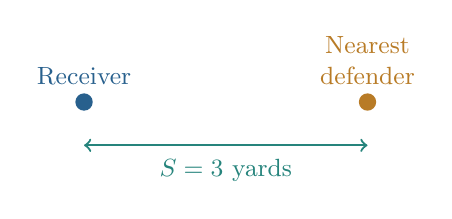
\begin{tikzpicture}[x=1cm,y=1cm]
\fill[blue] (0,0) circle (.11);
\fill[gold] (3.6,0) circle (.11);
\node[above,font=\small,text=blue] at (0,.1) {Receiver};
\node[above,font=\small,text=gold,align=center] at (3.6,.1) {Nearest\\defender};
\draw[<->,thick,teal] (0,-.55)--(3.6,-.55);
\node[below,font=\small,text=teal] at (1.8,-.6) {$S=3$ yards};
\end{tikzpicture}
\end{center}
This is a separate game illustration. Larger $S$ means more space at that instant; it does not guarantee a catch.\par\medskip
Use the same drill, time window and game moment for consistent comparisons.
\end{columns}
\note{The speed and distance examples are separate hypothetical illustrations, not paired data or a fitted relationship. Here v(t) is scalar speed at the candidate turn and t is measured in seconds. A speed rise from3to4yd/s over0.5s gives2yd/s2. Negative values are retained and indicate a lower endpoint speed, not deceleration at every instant. Consistent definitions alone do not establish that A measures a stable ability. Keep PLAYER tracks from the right-curl drill and group by player and event. Compare displacement headings0.5s before and after a candidate instant, require both displacement speeds at least2yd/s, angle at least45degrees and complete windows, then select the largest eligible angle. Take the median across eligible trials for each player;67players have one trial and one has two. The observed trajectory illustration has been removed from this slide. Two candidate events have been visually checked, but all69require review without selecting for a stronger outcome association. Candidate turn timing may precede speed recovery. S is the supplied nearest-defender distance at pass release; the drawing illustrates this definition and does not imply that A=2causes S=3. The regression asks whether player-level A is associated with repeated play-level S after accounting for sprint time and context.}
\end{frame}

\begin{frame}{Does the measurement window change the result?}
\small
Keep the same turn. Compare average speed change \textbf{per second} over 0.3, 0.5 and 0.7 s.\par
\key{Each dot is one receiver. The gray line means both windows give the same value.}\par
\begin{columns}[T,onlytextwidth]
\column{.49\textwidth}\centering
\begin{tikzpicture}\begin{axis}[base,width=6.55cm,height=3.05cm,
 title={Shorter window: 0.3 seconds},xmin=-3.5,xmax=6,ymin=-3.5,ymax=6,
 xlabel={0.5-s $A$ (yd/s$^2$)},ylabel={$A$ (yd/s$^2$)}]
\windowscatter{A03}
\end{axis}\end{tikzpicture}\par
\textbf{Median absolute change: 0.49 yd/s$^2$}
\column{.49\textwidth}\centering
\begin{tikzpicture}\begin{axis}[base,width=6.55cm,height=3.05cm,
 title={Longer window: 0.7 seconds},xmin=-3.5,xmax=6,ymin=-3.5,ymax=6,
 xlabel={0.5-s $A$ (yd/s$^2$)},ylabel={$A$ (yd/s$^2$)}]
\windowscatter{A07}
\end{axis}\end{tikzpicture}\par
\textbf{Median absolute change: 0.27 yd/s$^2$}
\end{columns}
\par
\begin{itemize}
\setlength{\itemsep}{0.7mm}
\item \textbf{Reading the plots:} near the line means similar values. Above means a larger value with the alternative window, and below means a smaller one.
\item \textbf{Decision:} player ordering is broadly similar. Keep 0.5 s and check the alternatives. Turn timing still needs review.
\end{itemize}
\note{A(w)=[s(t_cut+w)-s(t_cut)]/w. The same cut times, event set and filters are retained across windows, giving68players and69events throughout. Blue circles identify2023, teal triangles2024and gold squares2025. The colors consistently identify draft cohorts throughout the presentation. Median absolute change is the median across players of |A(w)-A(0.5)|. Spearman rank correlations are0.872856for0.3and0.944697for0.7; Pearson correlations are0.928630and0.966858. The same player is negative in all windows and no player changes sign. This conditional sensitivity check neither validates the cut point nor establishes test-retest reliability. No window is chosen using its association with NFL separation.}
\end{frame}

\begin{frame}{What the separation distribution tells us}
\small
\begin{columns}[T,onlytextwidth]
\column{.49\textwidth}\centering
\begin{tikzpicture}\begin{axis}[base,width=6.65cm,height=3.15cm,ybar interval,
 title={Original separation},xmin=0,xmax=18,ymin=0,ymax=5000,
 x tick label as interval=false,xlabel={Separation (yd)},ylabel={Records},xtick={0,4,8,12,16}]
\addplot[fill=blue,draw=white] table[x=edge,y=count,col sep=comma]{data/hist_raw.csv};
\end{axis}\end{tikzpicture}\par
\key{Skewness: 1.28}
\column{.49\textwidth}\centering
\begin{tikzpicture}\begin{axis}[base,width=6.65cm,height=3.15cm,ybar interval,
 title={Natural log separation},xmin=-1.5,xmax=3,ymin=0,ymax=3500,
 x tick label as interval=false,xlabel={$\log(S/1\,\mathrm{yd})$},ylabel={Records},xtick={-1,0,1,2,3}]
\addplot[fill=teal,draw=white] table[x=edge,y=count,col sep=comma]{data/hist_log.csv};
\end{axis}\end{tikzpicture}\par
\key{Skewness: $-0.20$}
\end{columns}
\vspace{1mm}
\small
\textbf{11,405 records:} mean 3.07 yd; median 2.61 yd; middle 50\%: 1.39--4.25 yd; range: 0.28--17.68 yd.
\begin{itemize}
\setlength{\itemsep}{1mm}
\item \textbf{Original scale:} a few large distances create a right tail and pull the mean above the median.
\item \textbf{Log scale:} compresses large distances; predictions convert back to positive distances in yards.
\item \textbf{Model choice:} fit Gaussian regression for $\log S$; check residual shape and spread after adjustment.
\end{itemize}
\note{All distributional summaries use the same68-player11405-record sample. The exact raw skewness is1.27756and log skewness-0.19927. Raw histogram bins are2yd wide and log bins0.5. A symmetric marginal histogram does not establish normal conditional residuals or constant variance, so posterior predictive checks remain necessary. Repeated plays are retained for distributional description, while the hierarchy addresses grouping in inference. The lognormal model gives positive predictive draws; exp(mu) is the conditional median, not generally the arithmetic or marginal mean.}
\end{frame}

\begin{frame}{Speed change, sprint time and NFL separation}
\small
\key{Purpose: see how $A$ relates to our sprint benchmark and NFL outcome.}\par
Each dot is one receiver. Colors show draft year:
\textcolor{blue}{2023}\quad\textcolor{teal}{2024}\quad\textcolor{gold}{2025}.
\vspace{2mm}\par
\begin{columns}[T,onlytextwidth]
\column{.49\textwidth}\centering
\key{1. Is $A$ related to sprint time?}\par\smallskip
\begin{tikzpicture}\begin{axis}[scatterbase,height=3.1cm,ymin=4.3,ymax=4.72,
 xlabel={Speed change $A$ (yd/s$^2$)},ylabel={40-yard time (s)},ytick={4.3,4.4,4.5,4.6,4.7}]
\cohortscatter{A}{forty}
\end{axis}\end{tikzpicture}\par
Little visible relationship with sprint time.\par
This alone does not establish $A$'s usefulness.
\column{.49\textwidth}\centering
\key{2. Is $A$ related to average space?}\par\smallskip
\begin{tikzpicture}\begin{axis}[scatterbase,height=3.1cm,ymin=1,ymax=8,
 xlabel={Speed change $A$ (yd/s$^2$)},ylabel={Mean $S$ (yd)},ytick={2,4,6,8}]
\cohortscatter{A}{mean_S}
\end{axis}\end{tikzpicture}\par
No clear upward trend in average space.\par
These averages mix different game contexts.
\end{columns}
\vspace{3mm}\par
\textbf{Next step:} compare models with and without $A$, controlling for sprint time and context. Report uncertainty even if $A$ adds little.
\note{These are descriptive checks before regression. A weak correlation with sprint time does not demonstrate an independent physical skill, measurement validity or predictive value. There are68equally weighted player points. The right chart uses arithmetic mean separation in yards from mean_S, not mean log separation. The subsequent regression still models log separation per play. Pearson r is-0.082225for A versus forty and-0.01830174for A versus mean_S. Players' averages have different precision because observation counts differ. A weak raw trend neither proves zero adjusted association nor guarantees a signal after adjustment. Compare the same finalized sample using grouped-by-player validation and report uncertainty rather than choosing specifications to obtain a positive result.}
\end{frame}

\begin{frame}{Why game context must enter the comparison}
\small
\key{Purpose: account for the situations receivers face before relating their separation to $A$.}
\vspace{2mm}\par
\begin{columns}[T,onlytextwidth]
\column{.43\textwidth}\centering
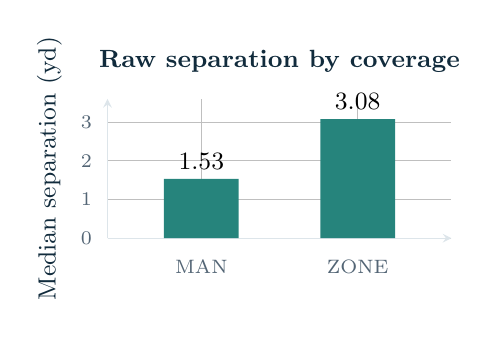
\begin{tikzpicture}\begin{axis}[base,ybar,width=5.95cm,height=3.35cm,
 title={Raw separation by coverage},symbolic x coords={MAN,ZONE},xtick=data,
 ymin=0,ymax=3.6,ylabel={Median separation (yd)},bar width=27pt,
 nodes near coords,nodes near coords style={font=\small},ytick={0,1,2,3},enlarge x limits=.6]
\addplot[fill=teal,draw=none] coordinates {(MAN,1.53) (ZONE,3.08)};
\end{axis}\end{tikzpicture}\par
MAN: 3,208 records. ZONE: 8,197.\par\smallskip\raggedright
Raw medians mix players, routes and other contexts.
\column{.54\textwidth}
\key{What else differs across plays?}\par\medskip
\textbf{Route:} the receiver's path and depth. A long straight run differs from a short route with a turn.\par\medskip
\textbf{Cushion:} the gap to a defender before the play starts. Receivers may begin with different amounts of space.\par\medskip
\textbf{Down and yards to go:} the attempt number and distance still needed for a first down.
\end{columns}
\vspace{2mm}\par
\textbf{Model decision:} include coverage and these context variables, so their associations with separation are accounted for when estimating $\beta_A$.
\note{The purpose is the choice of adjustment variables, not a ranking of receivers or a causal estimate of coverage. Coverage medians are1.526679and3.082402yd. All11405records yieldMAN3208andZONE8197. The raw difference can combine within-player coverage variation, player composition, route composition and other context. The model separates within-player MAN variation from usual MAN exposure. Route counts, previously shown as a table, are retained here:GO2393,HITCH1820,CROSS1377,IN1278,POST1244,OUT1119,CORNER903,SLANT734,SCREEN312,FLAT225. Counts alone do not establish route effects. Route categories are included because their paths and depths can differ, while the analysis estimates their adjusted associations. Pre-snap cushion is distance to the primary defender, who may not be the nearest defender at release. Context adjustment does not remove all unmeasured tactical, quarterback or selection differences.}
\end{frame}

\begin{frame}{Why the data call for a hierarchical model}
\small
The \textbf{11,405 records share 68 receivers and 559 games}. Plays from the same receiver or game can be related.
\begin{center}
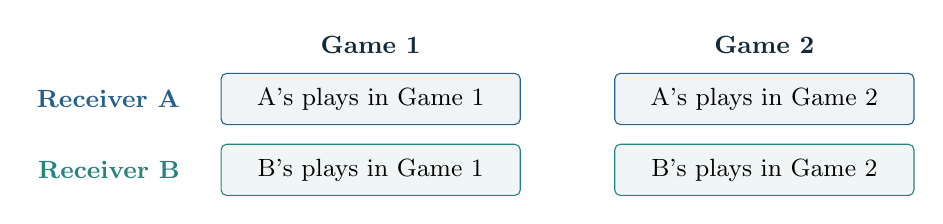
\begin{tikzpicture}[font=\small]
\node[font=\small\bfseries,text=ink] at (4,.18) {Game 1};
\node[font=\small\bfseries,text=ink] at (9,.18) {Game 2};
\node[anchor=east,text=blue,font=\small\bfseries] at (1.7,-.5) {Receiver A};
\node[anchor=east,text=teal,font=\small\bfseries] at (1.7,-1.4) {Receiver B};
\node[draw=blue,fill=blue!7,rounded corners=2pt,minimum width=3.8cm,minimum height=.65cm] at (4,-.5) {A's plays in Game 1};
\node[draw=blue,fill=blue!7,rounded corners=2pt,minimum width=3.8cm,minimum height=.65cm] at (9,-.5) {A's plays in Game 2};
\node[draw=teal,fill=teal!7,rounded corners=2pt,minimum width=3.8cm,minimum height=.65cm] at (4,-1.4) {B's plays in Game 1};
\node[draw=teal,fill=teal!7,rounded corners=2pt,minimum width=3.8cm,minimum height=.65cm] at (9,-1.4) {B's plays in Game 2};
\end{tikzpicture}
\end{center}
\begin{itemize}
\setlength{\itemsep}{2mm}
\item \textbf{Shared baselines:} player and game effects account for related observations. Ignoring these groups can make uncertainty look too small.
\item \textbf{A player-level question:} $A_i$ is fixed within a receiver. Its association with separation comes from comparing receivers.
\item \textbf{Unequal information:} players contribute 1--431 records. Partial pooling combines their own records with the expected baseline for players with similar measured characteristics.
\end{itemize}
\note{The player-by-game matrix is illustrative. Player and game effects are crossed because a receiver appears in several games and games contain several receivers. Additional plays inform player baselines and context but do not create new independent measurements of A. The hierarchy models player intercepts around a regression expectation using A, sprint time, coverage exposure and cohort. Pooling depends on uncertainty and between-player variation, not count alone. Other methods can also address dependence. Partial pooling does not remove confounding, and the68receivers should not be described as fully independent when games are shared.}
\end{frame}

\begin{frame}{Coverage has two roles in the model}
\small
Receivers face different mixes of MAN and ZONE. Separate \textbf{this play's coverage} from \textbf{the coverage a receiver usually faces}.
\vspace{3mm}\par
\begin{columns}[T,onlytextwidth]
\column{.48\textwidth}
\key{1. Compare the same receiver}\par\smallskip
Illustration: 25 of 100 plays are MAN.\par
The player's MAN share is $\bar M_i=0.25$.\par\smallskip
{\renewcommand{\arraystretch}{1.08}
\begin{tabular}{@{}lcc@{}}
\toprule
\textbf{This play} & $M$ & $M^W=M-\bar M_i$\\
\midrule
MAN & 1 & $0.75$\\
ZONE & 0 & $-0.25$\\
\bottomrule
\end{tabular}\par}
\smallskip
The difference is $0.75-(-0.25)=1$.\par\smallskip
$\lambda_W$ describes the MAN--ZONE log-separation contrast for the same receiver, with other context fixed.
\column{.49\textwidth}
\key{2. Compare usual exposure}\par\smallskip
Illustration: receiver A faces 25\% MAN, while receiver B faces 35\% MAN.\par\medskip
Do receivers who usually face more MAN have different adjusted baselines?\par\medskip
At each player's own usual coverage mix, the 10-point exposure gap contributes
\[
(0.35-0.25)\lambda_B=0.10\lambda_B
\]
to the expected log-separation baseline, with other player predictors fixed.
\end{columns}
\note{All numerical examples are hypothetical. Mbar is the proportion of eligible records coded MAN and remains on a0-to1scale. The within term M-Mbar changes by one for a same-player MAN--ZONE contrast. Lambda_B describes changes in the regression expectation of player intercepts at their respective average exposure, with A, forty and cohort fixed. It is not the between-player contrast holding the actual play's M fixed; that exposure contrast involves lambda_B-lambda_W. Random residual intercepts vary around their expectations. The decomposition does not identify a causal coverage effect or remove all confounding. Four players see only one coverage and have M^W=0on every record.}
\end{frame}

\begin{frame}{Main model: crossed player and game intercepts}
\small
For player $i$, play $p$, game $g$ and cohort $c(i)$, let $y_{ipg}=\log(S_{ipg}/1\,\mathrm{yd})$:
\begin{align*}
y_{ipg}&\sim N(\mu_{ipg},\sigma^2),\\
\mu_{ipg}&=\alpha_i+\lambda_W M^W_{ipg}
                  +\boldsymbol\gamma^T\mathbf W_{ipg}+u_g,\\[1mm]
\alpha_i&\sim N(m_i,\tau_{\mathrm{player}}^2),\\
m_i&=\alpha_0+\beta_A\Ai+\beta_F\Fi
                  +\lambda_B\bar M_i+\delta_{c(i)},\\
u_g&\sim N(0,\tau_{\mathrm{game}}^2).
\end{align*}
\key{$\mathbf W$: route, cushion, down, yards to go.}\par\medskip
$\Ai$ and $\Fi$ are standardized at the player level. Cohort effects use one reference category; player and game effects are crossed.
\note{The primary coefficient $\beta_A$ relates a player-level Combine measurement to repeated play-level outcomes. The player intercept is drawn around a regression mean, allowing partial pooling conditional on sprint time, speed change, coverage exposure and cohort. Player and game residual effects are independent in the initial model. The response is a log distance expressed numerically in yards. Game effects represent shared game variation and do not identify the causal contribution of any single game factor.}
\end{frame}

\begin{frame}{Model parameters: what each term means}
\small
$\mu_{ipg}$ is the expected \textbf{log separation}. SD means standard deviation.
\vspace{3mm}\par
\begin{columns}[T,onlytextwidth]
\column{.51\textwidth}
\key{Associations with log separation}\par\smallskip
{\renewcommand{\arraystretch}{1.12}
\begin{tabular}{@{}P{1.1cm}P{5.9cm}@{}}
$\beta_A$ & Change for a one-SD increase in $A$.\\
$\beta_F$ & Change for a one-SD longer sprint time (slower).\\
$\lambda_W$ & Same-player MAN--ZONE contrast.\\
$\lambda_B$ & Usual MAN share across receivers, at each receiver's own average exposure.\\
$\boldsymbol\gamma$ & Context coefficients for route, cushion, down and yards to go.\\
$\delta_c$ & Draft year versus reference year.\\
\end{tabular}\par}
\column{.46\textwidth}
\key{Baselines and standard deviations}\par\smallskip
{\renewcommand{\arraystretch}{1.12}
\begin{tabular}{@{}P{1.45cm}P{4.65cm}@{}}
$\alpha_0$ & Baseline at predictor zeros.\\
$m_i$ & Expected player baseline from measured characteristics.\\
$\alpha_i$ & Player baseline pooled toward $m_i$.\\
$u_g$ & Shared shift for game $g$.\\
$\tau_{\rm player}$ & Player spread around $m_i$.\\
$\tau_{\rm game}$ & Spread of game shifts.\\
$\sigma$ & Remaining play-level SD around $\mu_{ipg}$.\\
\end{tabular}\par}
\end{columns}
\vspace{2mm}\par
\textbf{Reading $\beta_A$:} $\exp(\beta_A)$ is the conditional median-separation ratio for a one-standard-deviation (SD) increase in $A$, with other inputs fixed.
\note{All additive baselines and regression coefficients are on the log-separation scale. Mu is a derived conditional mean of log separation, and m_i is the regression expectation of the player intercept, not a separately free coefficient. Neither m_i nor alpha_i is an observed player average. Alpha_0 is the reference intercept with standardized A and F at zero, MAN share at zero, reference draft cohort, and other coded mean components zero. Alpha_i is a player intercept drawn around m_i; u_g is a mean-zero game intercept. Tau_player and tau_game are SDs of random-effect distributions. Sigma is the residual SD of log outcomes. Beta_A describes a conditional between-player association, not a causal training effect. Beta_F is per1SDhigher forty time, which is slower performance. Gamma is a coefficient vector for play-context predictors. Lambda_W is the same-player MAN--ZONE contrast. Lambda_B compares expected baselines at players' own mean coverage exposure; a10percentage-point difference contributes0.1lambda_Bwith other player predictors fixed. Holding the actual play's MAN indicator fixed instead gives an exposure contrast involving lambda_B-lambda_W. Exp(beta_A)=1.10would mean a10percent higher conditional median for1SDhigher A, but this is only an illustration and no model has been fitted. Predictions in arithmetic mean yards require integrating uncertainty and are not generally exp(mu).}
\end{frame}

\begin{frame}{Implementation plan and expected deliverables}
\small\renewcommand{\arraystretch}{1.16}
\begin{tabular}{@{}P{1.1cm}P{6.5cm}P{5.0cm}@{}}
\toprule
\textbf{Stage} & \textbf{Work} & \textbf{Reviewable output}\\
\midrule
1 & Inspect all 69 trajectories; freeze filters, windows and final sample & Measurement audit; updated EDA\\
2 & Fit models with and without $A$; check priors and sampling & Coefficients, intervals and variance components\\
3 & Evaluate held-out players and posterior predictions & Predictive gains and calibration plots\\
4 & Check measurement and model sensitivity & Robustness table and limits of inference\\
\bottomrule
\end{tabular}\par
\vspace{2mm}
\key{Completed:} data joins, candidate-sample audit, descriptive EDA, and fixed-turn window sensitivity.\par\medskip
\key{Planned contribution:} quantify how much the trajectory metric adds beyond sprint time, with uncertainty at the player level.
\note{Sources: \url{https://www.kaggle.com/competitions/nfl-big-data-bowl-2027/data}; \url{https://sites.stat.columbia.edu/gelman/research/published/multi2.pdf}; \url{https://statmodeling.stat.columbia.edu/wp-content/uploads/2006/04/Bafumi_Gelman_Midwest06.pdf}; \url{https://mc-stan.org/loo/articles/online-only/faq.html}; \url{https://mc-stan.org/docs/stan-users-guide/regression.html}; \url{https://mc-stan.org/docs/stan-users-guide/posterior-predictive-checks.html}. Report weak or imprecise associations transparently. Final claims depend on measurement validation and model checks. The workflow is sequential: freeze the measurement before using outcome associations to assess it. If trajectory validation changes the sample, regenerate all EDA and compare models on the same final sample. The report should contain reproducible preprocessing, a variable dictionary, model specification, interval estimates, posterior predictive plots and grouped validation results. Do not claim model fitting is already complete.}
\end{frame}

\end{document}
